\documentclass[12pt, twoside]{article}
\usepackage[letterpaper, margin=1in, head=30pt, headsep=0.1in]{geometry}
\usepackage[english]{babel}
\usepackage[utf8]{inputenc}
\usepackage{amsmath}
\usepackage{amsfonts}
\usepackage{amssymb}
\usepackage{tikz}
%\usetikzlibrary{quotes, angles}

\usepackage{graphicx}
\usepackage{enumitem}
\usepackage{multicol}

\newif\ifmeta
\metatrue %print standards and topics tags

\title{Regents Geometry}
\author{Chris Huson}
\date{October 2021}

\usepackage{fancyhdr}
\pagestyle{fancy}
\fancyhf{}
\renewcommand{\headrulewidth}{0pt} % disable the underline of the header
\raggedbottom


\fancyhead[LE]{\thepage}
\fancyhead[RO]{\thepage \\ Name: \hspace{4cm} \,\\}
\fancyhead[LO]{BECA / Dr. Huson / Geometry 04 Analytic Geometry}

\begin{document}
\subsubsection*{4.7 Review: Transversal, Volume, Area}
\begin{enumerate}
\item The line $l$ is shown on the grid below.
\begin{multicols}{2}
\begin{enumerate}
  \item Write down it's slope, $y$-intercept.\\ $m=$
  \hspace{2cm} $b=$
  \vspace{0.25cm}
  \item Write down the equation of line $l$.
  \vspace{1cm}
  \item Draw a line parallel to line $l$ though point $S$.
  \item Write down the equation of the second line.
\end{enumerate}
  \begin{center}
  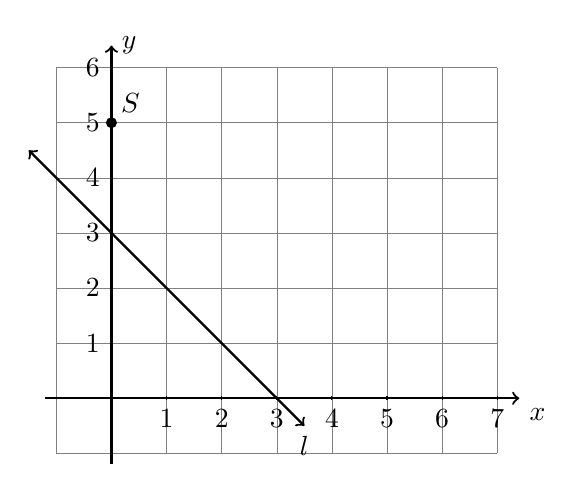
\begin{tikzpicture}[scale=0.7]
    \draw [help lines] (-1,-1) grid (7,6);
    \draw [thick, ->] (-1.2,0) -- (7.4,0) node [below right] {$x$};
    \draw [thick, ->] (0,-1.2)--(0,6.4) node [right] {$y$};
    \foreach \x in {1, ..., 7} \draw (\x cm,1pt) -- (\x cm,-1pt) node[anchor=north] {$\x$};
    \foreach \y in {1,...,6} \draw (1pt,\y cm) -- (-1pt,\y cm) node[anchor=east] {$\y$};
    \draw [thick, <->] (-1.5,4.5) -- (3.5,-0.5) node[below]{$l$};
    \fill (0,5) circle[radius=0.1] node[above right]{$S$};
  \end{tikzpicture}
  \end{center}
\end{multicols}\vspace{0.5cm}


\item Find the area $A$ and circumference $C$ of a circle with radius 5 feet (in terms of $\pi$). \vspace{3cm}

\item Find the area of the shape shown below composed of a rectangle and circular cap. Leave your answer as an exact value in terms of $\pi$.
\begin{flushright}
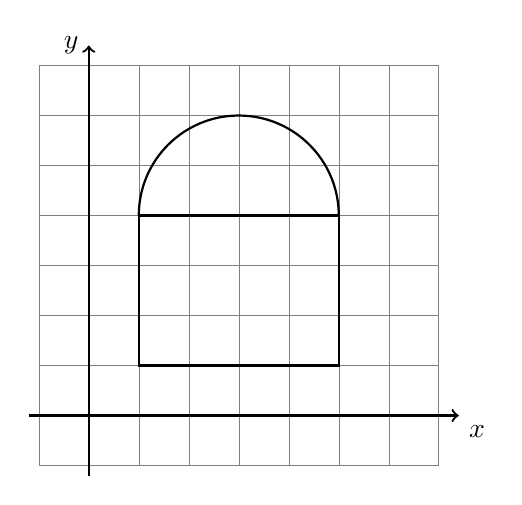
\begin{tikzpicture}[scale=.635]
  \draw [help lines] (-1,-1) grid (7,7);
  \draw [thick, ->] (-1.2,0) -- (7.4,0) node [below right] {$x$};
  \draw [thick, ->] (0,-1.2)--(0,7.4) node [left] {$y$};
  \draw [thick] (1,1)--(5,1)--(5,4)--(1,4)--cycle;
  %\draw [thick] (3,4) arc (90:270:1);
  \draw [thick] (5,4) arc (0:180:2);
\end{tikzpicture}
\end{flushright}

\newpage
\item A waffle cone has a radius of 2 inches and height of 4 inches. 
\begin{enumerate}
  \item Write down the general formula for the volume of a cone. \vspace{1cm}
  \item Find the volume of the waffle cone.
\end{enumerate}  \vspace{3cm}

\item Find $m\angle 1$ given two parallel lines and a transversal, with
  \begin{multicols}{2}
  $\displaystyle m\angle 1 = 2x+58$ \hspace{0.75cm}$\displaystyle m\angle 6 = 5x-18$
\begin{flushright}
  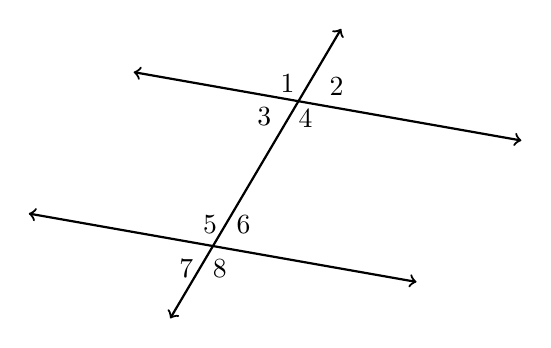
\begin{tikzpicture}[scale=1,rotate=-10]
    \draw [<->, thick] (3,2)--(8,2);
    \draw [<->, thick] (2,0)--(7,0);
    \draw [<->, thick] (4,-1)--(5.5,3);
    \node at (4.5,0.3) [left]{$5$};
    \node at (4.5,0.3) [right]{$6$};
    \node at (4.3,-0.3) [left]{$7$};
    \node at (4.3,-0.3) [right]{$8$};
    \node at (5.2,2) [above left]{$1$};
    \node at (5.4,2) [above right]{$2$};
    \node at (4.9,2) [below left]{$3$};
    \node at (5,2) [below right]{$4$};
  \end{tikzpicture}
\end{flushright} 
\end{multicols} \vspace{2cm}

\item An angle bisector is shown below, with $\overrightarrow{PR}$ bisecting $\angle QPS$. Given $m\angle QPR = 3x-12$ and $m\angle QPS = 5x+4$, find $m\angle QPS$.
    \begin{flushright}
    \begin{tikzpicture}[scale=0.6, rotate=30]
      \draw [<->, thick] (230:5)node[left]{$Q$} 
      --(0,0)node[above right]{$P$}
      --(110:6)node[above right]{$S$}--(110:7);
      \draw [->, thick] (0,0)--(170:7)node[below right]{$R$};
      %\draw [fill] (0,0) circle [radius=0.05] node[below]{$A$};
      %\draw [fill] (5,0) circle [radius=0.05] node[below]{$B$};
    \end{tikzpicture}
    \end{flushright}

\end{enumerate}
\end{document}



